% Chapter 14: Learning Regular Languages
% Sources: Course 89, L25-L26

\chapter{Learning Regular Languages}
\label{ch:learning-languages}

\aside{Chapter~\ref{ch:ctl-symbolic} ended our exploration of verification over known state sets. This chapter turns the question around: what if the state machine is a black box, and we must construct its model from external observations? We show how automata theory and machine learning meet via active learning.}

Up to this point, our verification algorithms assumed that the model of the system was given. We had a Kripke structure, an SMV file, or a set of multiset rewriting rules, and our task was to verify that it met a temporal logic specification or trace property. In practice, however, a complete model of a complex software system is rarely available. Often, we are confronted with a legacy implementation, a black-box hardware controller, or a third-party protocol whose internal state transitions are hidden.

This chapter introduces the technique of \emph{learning regular languages} (or automata learning). We bridge the gap between machine learning and formal language theory. Instead of learning continuous functions over fixed-dimensional real vectors (as in modern neural networks), our goal is to reconstruct the discrete structure of a finite-state machine by observing its input-output behavior. While this chapter focuses on deterministic finite automata, these active learning techniques have been successfully extended to probabilistic automata (e.g., for user profiling in systems like Amazon), tree automata for XML schema extraction, and tree transformations for modeling Linux package managers.

We follow the progression of the lecture block. We begin with the mathematical foundations of the Myhill--Nerode theorem, which guarantees that a regular language has a unique minimal representation. Then we transition to the active learning paradigm, explaining how a learner can reconstruct this minimal representation by asking targeted questions to a teacher. We describe Angluin's $L^*$ active-learning algorithm in detail, complete with a step-by-step trace on a concrete language and a formal proof of its correctness and complexity.

% =======================================================================
\section{The Myhill--Nerode Foundation}
\label{sec:myhill-nerode-learning}

The mathematical bridge that enables regular language learning is the Myhill--Nerode theorem. It provides a purely language-theoretic characterization of regular languages, independent of any automaton structure. This characterization is essential because a learner does not initially have access to states or transitions; it only observes whether specific strings belong to the target language.

\subsection{The equivalence relation}

Given a language $L \subseteq \Sigma^*$ over a finite alphabet $\Sigma$, we want to determine when two prefix strings $x$ and $y$ are ``equivalent'' from the perspective of $L$. Two prefixes are equivalent if they cannot be distinguished by any suffix extension.

\begin{definition}[Myhill--Nerode equivalence]
\label{def:myhill-nerode-equiv}
Let $L \subseteq \Sigma^*$ be a language. The Myhill--Nerode equivalence relation $\equiv_L \subseteq \Sigma^* \times \Sigma^*$ is defined as:
\[
  x \equiv_L y \iff \forall z \in \Sigma^*, (xz \in L \iff yz \in L)
\]
If $x \equiv_L y$, we say that $x$ and $y$ behave identically with respect to completions in $L$. We denote the equivalence class of a string $x$ by $[x]_L = \{y \in \Sigma^* \mid x \equiv_L y\}$.
\end{definition}

To simplify notation, we write $xz =_L yz$ to denote that $xz$ and $yz$ have the same membership status in $L$ (both inside or both outside). The relation $\equiv_L$ is an equivalence relation: it is reflexive, symmetric, and transitive. 

\begin{intermezzo}{The Puzzle Piece Analogy}
Imagine the universe of all strings $\Sigma^*$ painted on a canvas. The simplest classification is the trivial two-class equivalence: a blue region (strings inside $L$) and a gray region (strings outside $L$). The Myhill--Nerode equivalence classes act as \emph{puzzle pieces} that tile this canvas. 

Two critical properties govern these puzzle pieces:
\begin{enumerate}
    \item \textbf{Saturation}: A single puzzle piece cannot cross the blue/gray boundary. Every string in a piece must share the same membership status.
    \item \textbf{Right-invariance}: If you take all the strings in one puzzle piece and append the same letter $a$, they must all land squarely inside a \emph{single target puzzle piece}. You cannot split a puzzle piece by taking a step.
\end{enumerate}
\end{intermezzo}

Crucially, $\equiv_L$ satisfies the property of being a \emph{right congruence} (or being right invariant), perfectly matching our puzzle piece intuition.

\begin{lemma}[Right invariance]
\label{lem:right-invariance}
The equivalence relation $\equiv_L$ is right invariant. That is, for all $x, y \in \Sigma^*$ and all $a \in \Sigma$:
\[
  x \equiv_L y \implies xa \equiv_L ya
\]
\end{lemma}

\begin{proof}
Assume $x \equiv_L y$. By Definition~\ref{def:myhill-nerode-equiv}, this means that for all $z' \in \Sigma^*$, we have $xz' \in L \iff yz' \in L$. To show $xa \equiv_L ya$, we must show that for any suffix $z \in \Sigma^*$, $xaz \in L \iff yaz \in L$. This follows immediately by choosing $z' = az$ in the assumption.
\end{proof}

\subsection{Characterizing regular languages}

The Myhill--Nerode theorem states that the regularity of a language is completely determined by the number of equivalence classes (the index) of the relation $\equiv_L$.

\begin{theorem}[Myhill--Nerode]
\label{thm:myhill-nerode-learning}
A language $L \subseteq \Sigma^*$ is regular if and only if the equivalence relation $\equiv_L$ has a finite index (i.e., the quotient set $\Sigma^*/{\equiv_L}$ is finite).
\end{theorem}

Furthermore, if the index of $\equiv_L$ is finite and equal to $n$, then $n$ is exactly the number of states in the unique minimal deterministic finite automaton (DFA) recognizing $L$.

\begin{formaldetails}[Minimal DFA construction]
If $\equiv_L$ has a finite index, we can construct the canonical minimal DFA $A = (Q, \Sigma, \delta, q_0, F)$ recognizing $L$ directly from the equivalence classes:
\begin{itemize}
  \item \textbf{States}: $Q = \Sigma^*/{\equiv_L} = \{[w]_L \mid w \in \Sigma^*\}$. Since the index is finite, $Q$ is finite.
  \item \textbf{Initial State}: $q_0 = [\epsilon]_L$.
  \item \textbf{Transition Function}: $\delta([w]_L, a) = [wa]_L$ for all $w \in \Sigma^*$ and $a \in \Sigma$. (This is well-defined because if $[u]_L = [v]_L$, then $u \equiv_L v$, which implies $ua \equiv_L va$ by right invariance, meaning $[ua]_L = [va]_L$).
  \item \textbf{Final States}: $F = \{[w]_L \mid w \in L\}$. (This is well-defined because if $u \equiv_L v$ and $u \in L$, then by choosing the empty suffix $z = \epsilon$, we have $u\epsilon \in L \iff v\epsilon \in L$, hence $v \in L$).
\end{itemize}
\end{formaldetails}

\subsection{Examples of equivalence classes}

To clarify the intuition behind the Myhill--Nerode relation, we look at a non-regular language and a regular language.

\begin{example}[A non-regular language: Palindromes]
Let $\Sigma = \{a, b\}$ and let $L_{\text{pal}} = \{w \in \Sigma^* \mid w = w^R\}$ be the language of palindromes (strings that read the same backward and forward). We show that $\equiv_{L_{\text{pal}}}$ has an infinite index.

Consider two distinct strings $u, v \in \Sigma^*$ of the same length, say $u = ab$ and $v = bb$. To prove they belong to different equivalence classes, we must find a suffix $z$ that distinguishes them. Choose $z = a$ (the reverse of $u$).
\begin{itemize}
  \item $uz = aba \in L_{\text{pal}}$ (a palindrome).
  \item $vz = bba \notin L_{\text{pal}}$ (not a palindrome).
\end{itemize}
Since $uz \in L_{\text{pal}}$ but $vz \notin L_{\text{pal}}$, we have $u \not\equiv_{L_{\text{pal}}} v$. 

In general, for any two distinct strings $u \neq v$, if we choose the suffix $z = u^R$ (the reverse of $u$), then $uz = uu^R$ is always a palindrome. However, if $u$ and $v$ have different structures, $vu^R$ is not guaranteed to be a palindrome. In fact, each string $w \in \Sigma^*$ belongs to its own distinct equivalence class. Since $\Sigma^*$ is infinite, $\equiv_{L_{\text{pal}}}$ has an infinite index, which proves that the language of palindromes is not regular.
\end{example}

\begin{example}[A regular language: $L = ab^*$]
Let $\Sigma = \{a, b\}$ and $L = ab^* = \{a, ab, abb, abbb, \dots\}$. We determine the equivalence classes of $\equiv_L$:
\begin{enumerate}
  \item \textbf{Class 1: $[\epsilon]_L$}. Contains the empty string $\epsilon$. If we extend $\epsilon$ with a suffix $z$, the resulting string $z$ is in $L$ iff $z \in ab^*$.
  \item \textbf{Class 2: $[a]_L$}. Contains strings that have already matched the prefix $a$ and can be completed by any number of $b$'s. This class contains $\{a, ab, abb, \dots\}$, which is exactly the language $L$ itself. For any $w \in [a]_L$, extending it with $b$ keeps it in the class: $wb \in L$, whereas extending it with $a$ goes outside the language: $wa \notin L$.
  \item \textbf{Class 3: $[b]_L$}. Contains strings that start with the incorrect symbol $b$, making it impossible to ever complete them to form a string in $L$. This is a ``sink'' class containing $\{b, ba, bb, aa, aab, \dots\}$. For any string $w$ in this class and any suffix $z$, $wz \notin L$.
\end{enumerate}
Thus, there are exactly three equivalence classes: $[\epsilon]_L$, $[a]_L$, and $[b]_L$. Since the index is $3$, the minimal DFA recognizing $ab^*$ has exactly $3$ states.
\end{example}

% =======================================================================
\section{Passive vs. Active Learning}
\label{sec:active-learning}

In machine learning, we distinguish between different paradigms depending on how the learner interacts with the data source. The two primary paradigms are \emph{passive learning} and \emph{active learning}.

\subsection{Passive learning and its limitations}

In the classical passive learning model (such as Gold's identification in the limit), the learner is presented with a fixed set of training samples:
\[
  D = \{(x_1, y_1), (x_2, y_2), \dots, (x_m, y_m)\}
\]
where each $x_i \in \Sigma^*$ is a string and $y_i \in \{0, 1\}$ indicates whether $x_i \in L$. The learner's task is to find a DFA $A$ that is consistent with the dataset $D$ (i.e., $L(A)$ accepts $x_i$ iff $y_i = 1$).

Passive learning of regular languages has severe computational limitations:
\begin{itemize}
  \item \textbf{NP-completeness}: Finding the minimal DFA that is consistent with a given set of positive and negative examples is NP-complete (Gold, 1978).
  \item \textbf{Hardness of approximation}: It is computationally hard to approximate the minimal DFA within any polynomial factor unless $\text{P} = \text{NP}$.
\end{itemize}
This hardness arises because the learner is a passive recipient of the data. It cannot choose which parts of the state space to explore, leading to an exponential search space to resolve ambiguities.

\subsection{Active learning: The MAT framework}

To bypass these negative results, Dana Angluin (1987) proposed the \emph{active learning} paradigm. In this model, the information flow is two-way: the learner is not passive but can actively interact with an oracle called the \textbf{Minimally Adequate Teacher} (MAT). 

\begin{figure}[H]
  \centering
  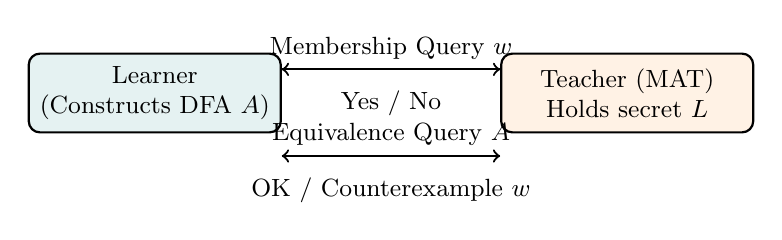
\begin{tikzpicture}[
      box/.style={draw, rounded corners, minimum width=3.2cm,
                  minimum height=1.0cm, align=center, font=\small, thick},
      arr/.style={->, thick}
    ]
    \node[box, fill=teal!10]  (learner) at (0,0) {Learner\\(Constructs DFA $A$)};
    \node[box, fill=orange!10] (teacher) at (6.0,0) {Teacher (MAT)\\Holds secret $L$};

    \draw[arr] ([yshift=3mm] learner.east) -- node[above, font=\small] {Membership Query $w$} ([yshift=3mm] teacher.west);
    \draw[arr] ([yshift=3mm] teacher.west) -- node[below=4pt, font=\small] {Yes / No} ([yshift=3mm] learner.east);

    \draw[arr] ([yshift=-8mm] learner.east) -- node[above, font=\small] {Equivalence Query $A$} ([yshift=-8mm] teacher.west);
    \draw[arr] ([yshift=-8mm] teacher.west) -- node[below=4pt, font=\small] {OK / Counterexample $w$} ([yshift=-8mm] learner.east);
  \end{tikzpicture}
  \caption{The Minimally Adequate Teacher (MAT) framework. The learner interacts with the teacher using two types of queries to iteratively refine its candidate DFA.}
  \label{fig:mat-framework}
\end{figure}

The active learning setup is often framed as a game between a \textbf{Learner} and a \textbf{Teacher}. The teacher holds a secret target regular language $L$ (represented internally as a DFA, regular expression, or black-box program). The learner only knows the alphabet $\Sigma$ and must reconstruct the minimal DFA for $L$. To do this, the learner can ask two types of queries. 

Could the learner win the game using only one type of query?
\begin{itemize}
    \item \textbf{Only Membership Queries?} No. If the learner only asks "is string $w$ in $L$?", it can only gather a finite set of labeled examples. There are always infinitely many valid DFAs that fit any finite set of points. The learner could never be mathematically certain it found the right one.
    \item \textbf{Only Equivalence Queries?} Yes! Since the set of all DFAs is countable, the learner could simply enumerate them ($A_1, A_2, A_3 \dots$) and ask "Is it $A_1$?", "Is it $A_2$?". The teacher will eventually say yes. However, this brute-force approach takes \emph{exponential time}.
\end{itemize}

By combining both queries, the MAT framework allows the learner to win the game in polynomial time.

\begin{definition}[Membership Query]
\label{def:membership-query}
In a \textbf{Membership Query (MQ)}, the learner presents a string $w \in \Sigma^*$ to the teacher. The teacher answers:
\[
  \text{MQ}(w) = 
  \begin{cases} 
    1 & \text{if } w \in L \\
    0 & \text{if } w \notin L
  \end{cases}
\]
\end{definition}

\begin{definition}[Equivalence Query]
\label{def:equivalence-query}
In an \textbf{Equivalence Query (EQ)}, the learner presents a candidate DFA $A$ to the teacher. The teacher checks whether $L(A) = L$.
\begin{itemize}
  \item If $L(A) = L$, the teacher replies \textbf{Yes} (or OK), and the learning process terminates successfully.
  \item If $L(A) \neq L$, the teacher replies \textbf{No} and provides a \textbf{counterexample} $w \in \Sigma^*$. The counterexample is in the symmetric difference of the two languages:
  \[
    w \in (L(A) \setminus L) \cup (L \setminus L(A))
  \]
\end{itemize}
\end{definition}

\begin{intermezzo}{The shortest counterexample requirement}
To prevent an adversarial teacher from stalling the algorithm by returning arbitrarily long counterexamples, we assume the teacher is honest and returns the \emph{shortest} possible counterexample. In practice, the shortest counterexample is polynomial in the size of the minimal DFA.
\end{intermezzo}

By combining MQs and EQs, active learning makes it possible to reconstruct the minimal DFA in polynomial time. The learner uses MQs to explore local state transitions and EQs to detect global discrepancies between the candidate model and the true language.

\medskip\noindent
\textbf{Approximating EQs in Practice.} The MAT framework is a theoretical ideal. In real-world system identification (often called ``model learning'' or ``black-box checking''), the teacher is not a mathematical oracle but a physical protocol or software system. While MQs are easy to execute (just send a test sequence to the system and observe if it accepts or crashes), EQs are impossible to answer perfectly. In practice, EQs are approximated via \textbf{fuzzing}: the learner launches large batches of random test sequences against both the physical system and the candidate DFA. If the outputs match for thousands of random tests, the learner assumes the candidate DFA is equivalent to the system. If a discrepancy is found, that specific test sequence serves as the counterexample.

% =======================================================================
\section{Angluin's $L^*$ Algorithm}
\label{sec:lstar-algorithm}

Angluin's $L^*$ algorithm organizes the learner's knowledge in a structured tabular format called the \textbf{observation table}. The algorithm maintains and updates two finite sets of strings over $\Sigma$:
\begin{itemize}
  \item $S \subset \Sigma^*$: The set of \textbf{state representatives}. These represent prefixes that lead to distinct states in the target DFA.
  \item $T \subset \Sigma^*$: The \textbf{test set} of suffixes. These are used to distinguish different state representatives.
\end{itemize}
Initially, $S = \{\epsilon\}$ and $T = \{\epsilon\}$.

\subsection{The observation table structure}

The observation table is a matrix where:
\begin{itemize}
  \item The rows are indexed by elements of the set $S \cup (S \cdot \Sigma)$, where $S \cdot \Sigma = \{s \cdot a \mid s \in S, a \in \Sigma\}$ represents the one-step extensions of our state representatives.
  \item The columns are indexed by elements of the test set $T$.
  \item The cell at row $s \in S \cup (S \cdot \Sigma)$ and column $t \in T$ is filled by querying the teacher via a Membership Query:
  \[
    \text{Table}(s, t) = \text{MQ}(s \cdot t) \in \{0, 1\}
  \]
\end{itemize}

\aside{In practice, the observation table also serves as a memoization cache: if a string's membership has already been queried, its result is stored, preventing redundant queries to the teacher.}

Before defining the row profile, we must formally introduce the \textbf{$T$-restricted equivalence} ($\equiv_{L,T}$). This relation sits strictly between the trivial 2-class equivalence (equal-L) and the true Myhill-Nerode equivalence ($\equiv_L$). 
Two strings are $T$-equivalent if they cannot be distinguished by any suffix from the set $T$:
\[
  x \equiv_{L,T} y \iff \forall t \in T, (xt \in L \iff yt \in L)
\]

\begin{intermezzo}{The Test Set as a Knob}
Think of the test set $T$ as a \emph{tuning knob}. When $T$ is small (e.g., just $\{\epsilon\}$), $\equiv_{L,T}$ is a very coarse approximation, yielding large, chunky puzzle pieces. As the learner discovers counterexamples, it adds strings to $T$, effectively "turning the knob." This refines the equivalence, shattering the large puzzle pieces into smaller, more precise ones, until the approximation perfectly aligns with the true Myhill-Nerode equivalence classes.
\end{intermezzo}

For any string $s \in S \cup (S \cdot \Sigma)$, we define its \textbf{row profile} $\text{row}(s)$ as the finite vector of boolean values indexed by $T$:
\[
  \text{row}(s) = \langle \text{Table}(s, t_1), \text{Table}(s, t_2), \dots, \text{Table}(s, t_{|T|}) \rangle
\]
The row profile is simply the characteristic function (a vector of 0s and 1s) representing the $\equiv_{L,T}$ equivalence class of $s$. If two strings have the same row profile, they currently reside in the same approximated puzzle piece.

\subsection{Table properties: Minimality and Completeness}

The algorithm relies on two structural properties of the observation table to decide whether a candidate DFA can be constructed:

\begin{definition}[$T$-minimality]
\label{def:t-minimality}
An observation table is \textbf{$T$-minimal} (or consistent) if no two distinct state representatives in $S$ have the same row profile:
\[
  \forall s_1, s_2 \in S, (\text{row}(s_1) = \text{row}(s_2) \implies s_1 = s_2)
\]
In puzzle piece terms, minimality means we have selected \emph{at most one representative string per puzzle piece}. There are no redundant states.
\end{definition}

\begin{definition}[$T$-completeness]
\label{def:t-completeness}
An observation table is \textbf{$T$-complete} if for every one-step extension $s \cdot a \in S \cdot \Sigma$ (where $s \in S$ and $a \in \Sigma$), there exists a state representative $s' \in S$ with the same row profile:
\[
  \forall s \in S, \forall a \in \Sigma, \exists s' \in S, (\text{row}(s \cdot a) = \text{row}(s'))
\]
In puzzle piece terms, completeness means that if any representative takes a step by one letter and lands in a new puzzle piece, \emph{that target puzzle piece must already have a designated representative in $S$}. If it doesn't, the table is incomplete, and we must promote the stray string to be the new representative for that piece.
\end{definition}

\subsection{DFA Construction}

When the observation table is both $T$-minimal and $T$-complete, the learner has enough information to construct a candidate DFA $A = (Q, \Sigma, \delta, q_0, F)$:
\begin{itemize}
  \item \textbf{States}: $Q = S$ (the state representatives themselves).
  \item \textbf{Initial State}: $q_0 = \epsilon$ (which is always in $S$).
  \item \textbf{Transition Function}: For any $s \in S$ and $a \in \Sigma$, we define $\delta(s, a) = s'$, where $s' \in S$ is the unique state representative such that:
  \[
    \text{row}(s \cdot a) = \text{row}(s')
  \]
  ($T$-completeness guarantees that such an $s'$ exists, and $T$-minimality guarantees that it is unique).
  \item \textbf{Final States}: $F = \{s \in S \mid \text{Table}(s, \epsilon) = 1\}$. (Since $\epsilon \in T$, we know whether $s \cdot \epsilon = s \in L$ directly from the table's first column).
\end{itemize}

\subsection{The $L^*$ loop}

The algorithm runs in a loop by executing three phases:
\begin{enumerate}
  \item \textbf{Phase 1: Make Complete}. If the table is not complete, find some $s \in S$ and $a \in \Sigma$ such that $\text{row}(s \cdot a) \neq \text{row}(s')$ for all $s' \in S$. Add $s \cdot a$ to $S$. Fill the new table rows using MQs. Repeat until the table is complete. (Note: adding $s \cdot a$ to $S$ preserves $T$-minimality because $s \cdot a$ has a row profile that was not present in $S$).
  \item \textbf{Phase 2: Propose Candidate}. Once the table is complete, construct the candidate DFA $A$ and submit it in an Equivalence Query (EQ) to the teacher.
  \item \textbf{Phase 3: Refine via Suffixes}. If the teacher returns a counterexample $w$, the learner refines its approximation by adding $w$ and all its suffixes to the test set $T$. Adding columns to the table splits equivalence classes, making the table incomplete again. The learner loops back to Phase 1.
\end{enumerate}

\begin{algorithm}[H]
\SetAlgoLined
\DontPrintSemicolon
\caption{Angluin's $L^*$ active-learning algorithm}
\label{alg:lstar}
$S \leftarrow \{\epsilon\}$; \quad $T \leftarrow \{\epsilon\}$\;
Initialize observation table using MQs for $S \cup (S \cdot \Sigma) \times T$\;
\While{true}{
  \While{table is not complete}{
    Find $s \in S, a \in \Sigma$ such that $\forall s' \in S, \text{row}(s \cdot a) \neq \text{row}(s')$\;
    $S \leftarrow S \cup \{s \cdot a\}$\;
    Update observation table using MQs for the new rows\;
  }
  Construct candidate DFA $A$ from $S$ and $T$\;
  \eIf{\text{EQ}(A) returns OK}{
    \Return $A$ (Learning completed successfully)\;
  }{
    Receive counterexample $w$ from the teacher\;
    $T \leftarrow T \cup \text{suffixes}(w)$\;
    Update observation table using MQs for the new columns\;
  }
}
\end{algorithm}

% =======================================================================
\section{Walkthrough with a Concrete Example}
\label{sec:lstar-walkthrough}

We trace the execution of the $L^*$ algorithm on a concrete language to show how the observation table evolves, how completeness is checked, and how counterexamples refine the test set.

Let the alphabet be $\Sigma = \{a, b\}$ and the target language be:
\[
  L = (ab)^* = \{\epsilon, ab, abab, ababab, \dots\}
\]
We start with $S = \{\epsilon\}$ and $T = \{\epsilon\}$.

\subsection{Iteration 1}

We initialize the table with $S = \{\epsilon\}$ and $S \cdot \Sigma = \{a, b\}$. We query the teacher with Membership Queries for the strings $\epsilon \cdot \epsilon = \epsilon$, $a \cdot \epsilon = a$, and $b \cdot \epsilon = b$.

\begin{table}[H]
  \centering
  \begin{tabular}{rcc}
    \toprule
    $S \cup (S \cdot \Sigma)$ & & $T = \{\epsilon\}$ \\
    \midrule
    $\epsilon$ & $(S)$ & $1$ \\
    \midrule
    $a$ & & $0$ \\
    $b$ & & $0$ \\
    \bottomrule
  \end{tabular}
  \caption{Observation table in Iteration 1.}
  \label{tab:iter1}
\end{table}

We check $T$-completeness:
\begin{itemize}
  \item The row profile of the representative is $\text{row}(\epsilon) = \langle 1 \rangle$.
  \item The row profiles of the extensions are $\text{row}(a) = \langle 0 \rangle$ and $\text{row}(b) = \langle 0 \rangle$.
  \item Neither $\text{row}(a)$ nor $\text{row}(b)$ matches any row profile in $S$. The table is \textbf{not complete}.
\end{itemize}
To resolve the incompleteness, we select the prefix $a$ and move it to the set of representatives.
Our sets become:
\[
  S = \{\epsilon, a\}, \quad S \cdot \Sigma = \{b, aa, ab\}
\]

\subsection{Iteration 2}

We update the table and fill the new rows using MQs. Note that $aa \notin L$ and $ab \in L$.

\begin{table}[H]
  \centering
  \begin{tabular}{rcc}
    \toprule
    $S \cup (S \cdot \Sigma)$ & & $T = \{\epsilon\}$ \\
    \midrule
    $\epsilon$ & $(S)$ & $1$ \\
    $a$ & $(S)$ & $0$ \\
    \midrule
    $b$ & & $0$ \\
    $aa$ & & $0$ \\
    $ab$ & & $1$ \\
    \bottomrule
  \end{tabular}
  \caption{Observation table in Iteration 2.}
  \label{tab:iter2}
\end{table}

We check $T$-completeness:
\begin{itemize}
  \item The representative profiles are $\text{row}(\epsilon) = \langle 1 \rangle$ and $\text{row}(a) = \langle 0 \rangle$.
  \item The extension profiles are:
  \begin{itemize}
    \item $\text{row}(b) = \langle 0 \rangle = \text{row}(a)$ (matched)
    \item $\text{row}(aa) = \langle 0 \rangle = \text{row}(a)$ (matched)
    \item $\text{row}(ab) = \langle 1 \rangle = \text{row}(\epsilon)$ (matched)
  \end{itemize}
  All extensions have a matching row profile in $S$. The table is \textbf{complete}.
\end{itemize}

Since the table is complete and minimal, we construct the first candidate DFA $A_1$:
\begin{itemize}
  \item \textbf{States}: $Q = \{q_\epsilon, q_a\}$.
  \item \textbf{Initial State}: $q_\epsilon$.
  \item \textbf{Final States}: $F = \{q_\epsilon\}$ (since $\text{Table}(\epsilon, \epsilon) = 1$).
  \item \textbf{Transitions}:
  \begin{align*}
    \delta(q_\epsilon, a) &= q_a \quad (\text{since } \text{row}(\epsilon \cdot a) = \text{row}(a)) \\
    \delta(q_\epsilon, b) &= q_a \quad (\text{since } \text{row}(\epsilon \cdot b) = \text{row}(b) = \text{row}(a)) \\
    \delta(q_a, a) &= q_a \quad (\text{since } \text{row}(a \cdot a) = \text{row}(aa) = \text{row}(a)) \\
    \delta(q_a, b) &= q_\epsilon \quad (\text{since } \text{row}(a \cdot b) = \text{row}(ab) = \text{row}(\epsilon))
  \end{align*}
\end{itemize}

\begin{figure}[H]
  \centering
  \begin{tikzpicture}[shorten >=1pt, node distance=2.5cm, on grid, auto, thick]
    \node[state, initial, accepting] (q0) {$q_\epsilon$};
    \node[state] (q1) [right=of q0] {$q_a$};
    \path[->]
      (q0) edge [bend left] node {$a, b$} (q1)
      (q1) edge [bend left] node {$b$} (q0)
           edge [loop right] node {$a$} (q1);
  \end{tikzpicture}
  \caption{Candidate DFA $A_1$ proposed at the end of Iteration 2.}
  \label{fig:dfa-iter2}
\end{figure}

The learner submits $A_1$ in an Equivalence Query. The teacher checks if $L(A_1) = (ab)^*$.
It finds that $A_1$ accepts the string $bb$ (since $\delta(q_\epsilon, b) = q_a$ and $\delta(q_a, b) = q_\epsilon$, which is accepting). However, $bb \notin L$. The teacher replies \textbf{No} and returns the counterexample:
\[
  w = bb
\]
The suffixes of $w$ are $\{\epsilon, b, bb\}$. Since $\epsilon$ is already in $T$, we add $\{b, bb\}$ to the test set:
\[
  T = \{\epsilon, b, bb\}
\]
Adding these columns will split the row profiles and distinguish states that were previously merged.

\subsection{Iteration 3}

We reconstruct the observation table with the new column suffixes. The sets are $S = \{\epsilon, a\}$, and extensions $S \cdot \Sigma = \{b, aa, ab\}$. We query MQs to fill the cells.

\begin{table}[H]
  \centering
  \begin{tabular}{rcccc}
    \toprule
    $S \cup (S \cdot \Sigma)$ & & $\epsilon$ & $b$ & $bb$ \\
    \midrule
    $\epsilon$ & $(S)$ & $1$ & $0$ & $0$ \\
    $a$ & $(S)$ & $0$ & $1$ & $0$ \\
    \midrule
    $b$ & & $0$ & $0$ & $0$ \\
    $aa$ & & $0$ & $0$ & $0$ \\
    $ab$ & & $1$ & $0$ & $0$ \\
    \bottomrule
  \end{tabular}
  \caption{Observation table in Iteration 3.}
  \label{tab:iter3}
\end{table}

We check $T$-completeness:
\begin{itemize}
  \item The representative profiles are $\text{row}(\epsilon) = \langle 1, 0, 0 \rangle$ and $\text{row}(a) = \langle 0, 1, 0 \rangle$.
  \item The extension profiles are:
  \begin{itemize}
    \item $\text{row}(b) = \langle 0, 0, 0 \rangle$ (no match in $S$)
    \item $\text{row}(aa) = \langle 0, 0, 0 \rangle$ (no match in $S$)
    \item $\text{row}(ab) = \langle 1, 0, 0 \rangle = \text{row}(\epsilon)$ (matched)
  \end{itemize}
  The extension $b$ has a row profile $\langle 0, 0, 0 \rangle$ that is not present in $S$. The table is \textbf{not complete}.
\end{itemize}
We add the prefix $b$ to the set of representatives:
\[
  S = \{\epsilon, a, b\}, \quad S \cdot \Sigma = \{aa, ab, ba, bb\}
\]

\subsection{Iteration 4}

We fill the new rows for $ba$ and $bb$. Since they both start with $b$, any extension of them will also start with $b$ and can never belong to $L = (ab)^*$. Thus, all their suffix extensions are $0$.

\begin{table}[H]
  \centering
  \begin{tabular}{rcccc}
    \toprule
    $S \cup (S \cdot \Sigma)$ & & $\epsilon$ & $b$ & $bb$ \\
    \midrule
    $\epsilon$ & $(S)$ & $1$ & $0$ & $0$ \\
    $a$ & $(S)$ & $0$ & $1$ & $0$ \\
    $b$ & $(S)$ & $0$ & $0$ & $0$ \\
    \midrule
    $aa$ & & $0$ & $0$ & $0$ \\
    $ab$ & & $1$ & $0$ & $0$ \\
    $ba$ & & $0$ & $0$ & $0$ \\
    $bb$ & & $0$ & $0$ & $0$ \\
    \bottomrule
  \end{tabular}
  \caption{Observation table in Iteration 4.}
  \label{tab:iter4}
\end{table}

We check $T$-completeness:
\begin{itemize}
  \item The representative profiles are $\text{row}(\epsilon) = \langle 1, 0, 0 \rangle$, $\text{row}(a) = \langle 0, 1, 0 \rangle$, and $\text{row}(b) = \langle 0, 0, 0 \rangle$.
  \item The extension profiles are:
  \begin{itemize}
    \item $\text{row}(aa) = \langle 0, 0, 0 \rangle = \text{row}(b)$ (matched)
    \item $\text{row}(ab) = \langle 1, 0, 0 \rangle = \text{row}(\epsilon)$ (matched)
    \item $\text{row}(ba) = \langle 0, 0, 0 \rangle = \text{row}(b)$ (matched)
    \item $\text{row}(bb) = \langle 0, 0, 0 \rangle = \text{row}(b)$ (matched)
  \end{itemize}
  All extensions have a matching row profile in $S$. The table is \textbf{complete}.
\end{itemize}

We construct the second candidate DFA $A_2$:
\begin{itemize}
  \item \textbf{States}: $Q = \{q_\epsilon, q_a, q_b\}$.
  \item \textbf{Initial State}: $q_\epsilon$.
  \item \textbf{Final States}: $F = \{q_\epsilon\}$.
  \item \textbf{Transitions}:
  \begin{align*}
    \delta(q_\epsilon, a) &= q_a \quad (\text{since } \text{row}(\epsilon \cdot a) = \text{row}(a)) \\
    \delta(q_\epsilon, b) &= q_b \quad (\text{since } \text{row}(\epsilon \cdot b) = \text{row}(b)) \\
    \delta(q_a, a) &= q_b \quad (\text{since } \text{row}(a \cdot a) = \text{row}(b)) \\
    \delta(q_a, b) &= q_\epsilon \quad (\text{since } \text{row}(a \cdot b) = \text{row}(\epsilon)) \\
    \delta(q_b, a) &= q_b \quad (\text{since } \text{row}(b \cdot a) = \text{row}(b)) \\
    \delta(q_b, b) &= q_b \quad (\text{since } \text{row}(b \cdot b) = \text{row}(b))
  \end{align*}
\end{itemize}

\begin{figure}[H]
  \centering
  \begin{tikzpicture}[shorten >=1pt, node distance=2.5cm, on grid, auto, thick]
    \node[state, initial, accepting] (q0) {$q_\epsilon$};
    \node[state] (q1) [right=of q0] {$q_a$};
    \node[state] (q2) [below=of q1] {$q_b$};
    \path[->]
      (q0) edge [bend left] node {$a$} (q1)
           edge node [left] {$b$} (q2)
      (q1) edge [bend left] node {$b$} (q0)
           edge node [right] {$a$} (q2)
      (q2) edge [loop right] node {$a, b$} (q2);
  \end{tikzpicture}
  \caption{Candidate DFA $A_2$ proposed at the end of Iteration 4.}
  \label{fig:dfa-iter4}
\end{figure}

The learner submits $A_2$ to the teacher in an Equivalence Query. The teacher checks if $L(A_2) = (ab)^*$. Since $A_2$ is isomorphic to the minimal DFA for $(ab)^*$ (with $q_b$ as the sink state), the teacher replies \textbf{Yes}. The algorithm terminates successfully.

% =======================================================================
\section{Correctness, Termination, and Complexity}
\label{sec:lstar-correctness}

To establish the utility of the $L^*$ algorithm, we must prove that it is guaranteed to terminate with the correct minimal DFA, and that it does so using a polynomial number of queries.

\subsection{Complexity bounds}

Let $n$ be the number of states of the unique minimal DFA recognizing the target language $L$, and let $m$ be the maximum length of any counterexample returned by the teacher during equivalence queries.

\begin{itemize}
  \item \textbf{Size of $S$}: Since the observation table is maintained $T$-minimal, the set of representatives $S$ contains at most one string for each equivalence class. By Theorem~\ref{thm:myhill-nerode-learning}, the number of equivalence classes is $n$. Therefore, $|S| \le n$.
  \item \textbf{Number of Equivalence Queries}: Each time we fail an equivalence query, we add suffixes of the counterexample to $T$. We will prove below that this forces the addition of at least one new representative to $S$ in the next iteration. Since $|S|$ starts at $1$ and cannot exceed $n$, the algorithm can perform at most $n-1$ unsuccessful equivalence queries. Thus, the total number of equivalence queries is at most $n$.
  \item \textbf{Size of $T$}: We start with $T = \{\epsilon\}$. Each of the at most $n-1$ counterexamples has length at most $m$, contributing at most $m$ suffixes. Thus, $|T| \le 1 + (n-1)m$.
  \item \textbf{Number of Membership Queries}: The size of the observation table is $(|S| + |S| \cdot |\Sigma|) \times |T|$. Since $|S| \le n$ and $|T| \le nm$, the table has at most $n(1 + |\Sigma|) \cdot nm = \mathcal{O}(|\Sigma| n^2 m)$ cells. Each cell requires one Membership Query, so the total number of MQs is polynomial in $n$, $m$, and $|\Sigma|$.
\end{itemize}

\subsection{Proof of correctness and termination}

The key to the termination proof is showing that a counterexample really does force a state split. If we add the suffixes of a counterexample $w$ to $T$, the table cannot remain complete without introducing a new state representative.

\begin{formaldetails}[Proof roadmap: Counterexample state split]
Let $A$ be the candidate DFA constructed from a complete and minimal table $(S, T)$ in Phase 2. Suppose $A$ is incorrect, and the teacher returns a counterexample $w = a_1 a_2 \dots a_k$ of length $k \le m$.

Let $T' = T \cup \text{suffixes}(w)$ be the updated test set, where $\text{suffixes}(w) = \{t_0, t_1, \dots, t_k\}$ and each suffix is defined as:
\[
  t_i = a_{i+1} a_{i+2} \dots a_k \quad (\text{with } t_k = \epsilon, \, t_0 = w)
\]
We define the sequence of states $s_0, s_1, \dots, s_k \in S$ reached by the candidate DFA $A$ when processing the prefixes of $w$. Specifically, for each $i \in \{0, \dots, k\}$, let:
\[
  s_i = \delta^*(q_\epsilon, a_1 \dots a_i)
\]
where $s_0 = \epsilon$ and $s_i$ is the representative of the state reached after consuming prefix $a_1 \dots a_i$.

We assume, for the sake of contradiction, that the table remains $T'$-complete with the same set of representatives $S$. That is, no new representatives are added.

The most unintuitive---yet brilliant---step of this proof involves the string $s_i t_i$. Why this string? Think of it operationally: we feed the counterexample $w$ into the automaton, but we \emph{pause} it after reading the prefix $a_1 \dots a_i$. At this point, the automaton is in state $s_i$. We then \emph{swap out} the prefix we just read for the canonical string representative $s_i$, and \emph{play} the remaining suffix $t_i$. By tracking the membership of this hybrid string $s_i \cdot t_i$ as $i$ goes from $0$ to $k$, we can pinpoint exactly where the candidate automaton made a faulty transition. Under the assumption of completeness, we prove by induction that for all $i \in \{0, \dots, k\}$, the string $s_i \cdot t_i$ has the same membership status in $L$:
\[
  s_i t_i \in L \iff s_{i+1} t_{i+1} \in L
\]
For the inductive step, consider any $i \in \{0, \dots, k-1\}$. By definition, the transition of $A$ from state $s_i$ on symbol $a_{i+1}$ goes to state $s_{i+1}$:
\[
  \delta(s_i, a_{i+1}) = s_{i+1}
\]
By the construction of the DFA's transition function (Section~\ref{sec:lstar-algorithm}), this transition is well-defined because:
\[
  \text{row}_{T}(s_i \cdot a_{i+1}) = \text{row}_{T}(s_{i+1})
\]
Since we assumed the table remains complete under $T'$, we must have:
\[
  \text{row}_{T'}(s_i \cdot a_{i+1}) = \text{row}_{T'}(s_{i+1})
\]
This equality implies that for all suffixes $t \in T'$:
\[
  (s_i a_{i+1}) t \in L \iff s_{i+1} t \in L
\]
Since $t_{i+1}$ is a suffix of the counterexample $w$, we have $t_{i+1} \in T'$. Choosing $t = t_{i+1}$ yields:
\[
  s_i a_{i+1} t_{i+1} \in L \iff s_{i+1} t_{i+1} \in L
\]
Since $a_{i+1} t_{i+1} = t_i$, we obtain:
\[
  s_i t_i \in L \iff s_{i+1} t_{i+1} \in L
\]
By induction from $i = 0$ to $k$, we obtain:
\[
  s_0 t_0 \in L \iff s_1 t_1 \in L \iff \dots \iff s_k t_k \in L
\]
Now we evaluate the endpoints of this chain:
\begin{itemize}
  \item \textbf{Left-hand side}: $s_0 t_0 = \epsilon \cdot w = w$.
  \item \textbf{Right-hand side}: $s_k t_k = s_k \cdot \epsilon = s_k$.
\end{itemize}
Thus, we have:
\[
  w \in L \iff s_k \in L
\]
However, $s_k$ is the final state reached by $A$ when reading $w$. By the construction of final states in $A$, $s_k$ is a final state ($s_k \in F$) if and only if $s_k \in L$. Therefore, $A$ accepts $w$ if and only if $s_k \in L$, which is true if and only if $w \in L$.

This implies that $A$ accepts $w$ if and only if $w \in L$, which means $A$ correctly classifies the counterexample $w$. This directly contradicts the fact that $w$ is a counterexample ($w \in L(A) \iff w \notin L$).

This contradiction shows that the assumption of $T'$-completeness with the same set $S$ must be false. Therefore, adding the suffixes of $w$ to $T$ must break the completeness of the table, forcing the algorithm to add at least one new state representative to $S$ in the next iteration. Since the size of $S$ is bounded by $n$, the algorithm must terminate.
\end{formaldetails}



